\documentclass[sigplan,10pt]{acmart}
\renewcommand\footnotetextcopyrightpermission[1]{}
\pagestyle{plain}

% main conference info (commented for initial submission):
\copyrightyear{2019}
\acmYear{2019}
\setcopyright{acmlicensed}
\acmConference[SOSP '19]{SOSP '19: ACM Symposium on Operating Systems Principals}{October 27--30, 2019}{Huntsville, Ontario}


% not sure if we need this stuff:
% \acmBooktitle{Huntsville '19: ACM Symposium on Operating Systems Principals, October 27--30, 2019, Huntsville, Ontario}
%\acmPrice{15.00}
%\acmDOI{10.1145/1122445.1122456}
%\acmISBN{978-1-4503-9999-9/18/06}

% math
\usepackage{amsmath}

% multicolumn in tables
\usepackage{makecell}

% subfigure
\usepackage{subcaption}

% code
\usepackage{listings}

% enum indent control
\usepackage{enumitem}

 %tables
\usepackage{booktabs} 



\usepackage[T1]{fontenc}
\usepackage[scaled]{beramono}

\newcommand\SmallSz{\fontsize{8}{8.2}\selectfont}
\newcommand*\LSTfont{\SmallSz\ttfamily\SetTracking{encoding=*}{-60}\lsstyle}


%modern code fonts (this makes \sum disappear)
%\usepackage{lmodern}

\newcommand{\tc}[1]  {{\ttfamily\fontseries{m}\selectfont #1}}

% Note Macros:
\definecolor{mred}{rgb}{.80,.12,.30}
\definecolor{grey}{rgb}{0.5,0.5,0.5}
\definecolor{purple2}{rgb}{.75,0,.85}
\definecolor{pistachio}{rgb}{0.58, 0.77, 0.45}
\newcommand{\suman}[1]{\textcolor{mred}{(Suman: #1)}}
\newcommand{\gabe}[1] {\textcolor{purple2}{(Gabe: #1)}}
\newcommand{\abhi}[1] {\textcolor{blue}{(Abhi: #1)}}
\newcommand{\ksb}[1]  {\textcolor{pistachio}{(Koustubha: #1)}}
\newcommand{\dongdong}[1]  {\textcolor{pistachio}{(Dongdong: #1)}}

  %basicstyle=\footnotesize \ttfamily,

\lstset{
  basicstyle=\LSTfont,
  frame=single,
  showlines=true
}


%-------------------------------------------------------------------------------
\begin{document}
%-------------------------------------------------------------------------------

%don't want date printed
%\date{}

% make title bold and 14 pt font (Latex default is non-bold, 16 pt)
%\title{ Proximal Gradient Analysis for Systems Security}
\title{    Accurate Dynamic Data Flow Analysis with \\ Proximal Gradients}

%\author{ Author1}
%\email{email1@email.edu}

%\affiliation{%
  %\institution{Univerisity}
  %\streetaddress{StreetAddress}
  %\city{City}
  %\state{State}
  %\postcode{Zip}
%}

%\author{Author2}
%\email{email2@email.edu}

%\affiliation{%
  %\institution{Univerisity}
  %\streetaddress{StreetAddress}
  %\city{City}
  %\state{State}
  %\postcode{Zip}
%}
%%-------------------------------------------------------------------------------
\begin{abstract}
%-------------------------------------------------------------------------------
  \gabe{update abstract to be in line with intro}

Discovery of new security vulnerabilities is a fundamentally difficult problem because the space of possible inputs to a program is exponentially large. However, the parts of program input that significantly effect program behavior are sparse, so being able to correctly identify which parts of the input drive program behavior is key to effectively searching for vulnerabilities. To address this problem, several recent fuzzers have used dynamic taint tracking, or taint tracking, to track which input bytes have taint to branch variables or system calls. However, taint tracking is imprecise, having to either over or under approximate many operations, and only provides limited information about program behavior.

We introduce a novel form of program analysis, Proximal Gradient Analysis, that not only provides much more precise dataflow information than taint tracking, but also more overall information about program behavior in the form of a gradient. First, we provide a theoretical grounding for Proximal Gradient Analysis in Nonsmooth Optimization methods, and derive sampling bounds that enable principled evaluation of Proximal Gradients on nonsmooth operations. We then describe a methodology for evaluating Proximal Gradients over programs and a proof of concept implementation as an LLVM pass. Finally, we evaluate Proximal Gradient Analysis in comparison to taint tracking and show that it is able to identify dataflows to branch variables with X\% higher precision and produces Y\% higher branch coverage in dataflow guided fuzzing. Using Proximal Gradient Analysis as a guide, we were able to find Z\% new bugs in 7 widely used file parsing programs, including memory allocation errors, memory corruption errors, and undefined behavior errors.
\end{abstract}




% commented for initial submission
%\begin{CCSXML}
%<ccs2012>
%<concept>
%<concept_id>10002978.10003022.10003023</concept_id>
%<concept_desc>Security and privacy~Software security engineering</concept_desc>
%<concept_significance>500</concept_significance>
%</concept>
%</ccs2012>
%\end{CCSXML}
%\ccsdesc[500]{Security and privacy~Software security engineering}
%\keywords{Dataflow Analysis, Program Security, Vulnerability Detection, Gradient Analysis, Deep Learning}


\maketitle

%%-------------------------------------------------------------------------------
\section{Introduction}
%%-------------------------------------------------------------------------------
Dataflow analysis is a fundamental technique in software enginering that tracks which variables can influence each other and how information flows through a program ~\cite{kildall1973unified, fosdick2011data}. For security applications, a type of dataflow analysis called taint tracking is typically used, which tracks dataflows between a specified set of sources and sinks in a program ~\cite{newsome2005dynamic}. Taint tracking has multiple applications in security, including detecting attacks at run time, guided fuzzing, discovering information leaks, and malware analysis ~\cite{clause2007dytan, schwartz2010all, ganesh2009taint, rawat2017vuzzer, arzt2014flowdroid, yan2012droidscope}. It can be performed either statically, by analyzing the source code or binary of a program, or dynamically, by instrumenting a program and tracking taint as it executes. However, static analysis cannot distinguish invalid program states that cannot be reached during execution, leading to high false positive rates ~\cite{jovanovic2006pixy}. Dynamic taint analysis avoids this problem by operating on concrete executions, but still suffers from two limitations: it uses overapproximations in its propogation rules that still lead to high false positive rates, and it only operates on individual inputs, providing no information about overall program behavior ~\cite{balzarotti2008saner}. 

The overappoximations in dynamic taint tracking come from two sources: numerical errors on single instructions, and compound errors involving multiple instructions. Numerical errors occur when instructions inputs may or may not effect the output depending on their values. For example, in the operation \tc{y = x1 - x2;} both \tc{x1} and \tc{x2}  clearly effect the output \tc{y}, leading to the propogation rule $taint(y) = taint(x1) \cup taint(x2)$, but if the operation happens on the same variable \tc{y = x - x} this propogation will be incorrect. Compound errors occur when taint is propogated over sequence of operations that are handled correctly individually but incorrect in aggregate. In the two operations \tc{a = x1 + x2; b = a - x1;}, a taint propogation will indicate $taint(b) = taint(x1) \cup taint(x2)$, when in fact the value of $x1$ has no effect on $b$, and $taint(b) = taint(x2)$. The combined effect of these errors is that entire sections of a program will be incorrectly tainted during execution, making dynamic taint tracking impractical for most real world applications. \gabe{should we mention underapproximations from memory etc here too? We could argue we can address it with sampling, but it isn't implemented yet...}


%\begin{figure}
  %\centering
  %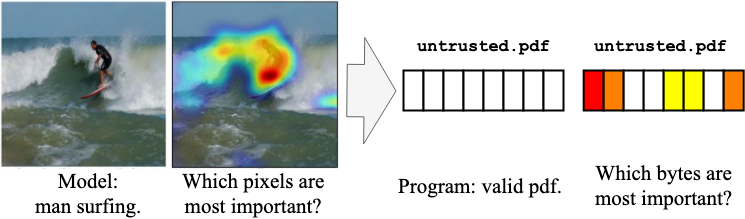
\includegraphics[width=\linewidth]{figs/sosp-nn_explain2}
  %\vspace{-15pt}
  %\caption{\label{fig:nn_analogy} Examples of gradient based explanations for machine learning model and program behavior ~\cite{selvaraju2017grad}.}
  %\vspace{-15pt}
%\end{figure}


To address these limitations, we draw inspiration from the fields of statistical modeling and optimization, in which gradients have long been used as a method for analyzing model behavior ~\cite{cook1986assessment}. Recently, gradients have been used for a variety of tasks that are analagous to dataflow analysis on programs, such as explaining model behavior, generating adversarial examples, and maximizing test coverage  ~\cite{baehrens2010explain, simonyan2013deep, shrikumar2017learning, goodfellow2014explaining, pei2017deepxplore}. In these applications, gradients serves as a measure of how inputs to a model determine its behavior, making it possible to explain that behavior or generate new inputs that alter the behavior. Dataflow in programs is similarly used to identify important inputs, discover vulnerabilities, and measure test coverage ~\cite{ganesh2009taint, rawat2017vuzzer, newsome2005dynamic, hutchins1994experiments}. 

%To address these limitations, we draw inspiration from the deep learning community, where accurately identifying which inputs explain why a model made a given decision is an active area of research. Conceptually, explaining model decisions is a dataflow problem, in which the input data that most strongly affects the model decision, and therefore flows to the output, should be identified. Many of these explanation methods rely on local gradient with regard to input, which is the slope of the model, or the measure of how change in the input changes the output for a given input ~\cite{baehrens2010explain, simonyan2013deep, shrikumar2017learning}. Intuitively, gradient serves as indication of how inputs effect outputs for differentiable models.



As a method for dataflow analysis, tracking gradients between variables within a program can address both limitations of taint tracking. In cases where taint would over approximate due to numerical or compound errors, such as operations like \tc{y = x - x;} the gradient $\tfrac{dy}{dx}$ is naturally $0$, so no overapproximation will occur. Moreover, gradient gives additional information by indicating how each of the source variables effect a given sink, which can be used to identify which sources are most significant or guide a search for vulnerabilities. Figure \ref{fig:taint_v_gradient} shows how these advantages can combine to cut out false positives and distinguish the most important inputs that can trigger a specific error in a program.


\begin{figure}
  \centering
  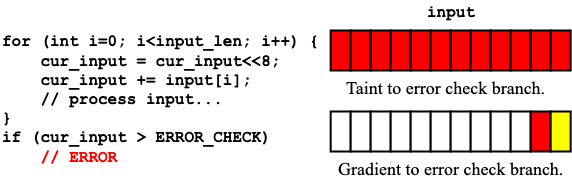
\includegraphics[width=\linewidth]{figs/sosp-grad_v_taint_ex}
  \vspace{-25pt}
  \caption{\label{fig:taint_v_gradient} Example of a program in which an iterated shift operation on the input will cause overtainting, while gradient will correctly identify which input bytes are most influential in triggering an error. \gabe{can change colors if this looks too much like a firetruck}}
  \vspace{-15pt}
\end{figure}

However, gradients cannot be computed over programs in the same way they are on continuous systems. In a continuous system, each operation is differentiable, so the gradients of individual operations can be composed via the chain rule to compute a gradient over the entire model ~\cite{Wengert:1964:SAD:355586.364791}. In contrast, programs contain many operations that are discrete and have nonsmooth behavior, such as bitwise operators and branches, which cannot be differentiated directly \gabe{should we just say nondifferentiable instead of nonsmooth? nonsmooth may be confusing.}. These nondifferentiable operations break the chain rule and prevent the gradient from being computed. Therefore, in order to evaluate gradients over programs, we use methods developed for nonsmooth optimization that relax the chain rule to apply to nondifferentiable functions. In particular, we use proximal gradients, a type of gradient approximation that is widely used to solve optimization problems with nondifferential objective functions ~\cite{parikh2014proximal}. 

Proximal gradients estimate the local gradient by finding a nearby minima of a function and drawing a line to it. They have two properties that make them well suited to working with nonsmooth operations in programs. First, they are robust to the discrete and nonsmooth behavior that makes program operations nondifferentiable, such that performing optimization with proximal gradients is proven to find a local minimum ~\cite{bertsekas2015convex}. Second, proximal gradients use a soft bound to limit the region in which they operate, making it possible to evaluate them without sampling all possible inputs to a function. 

To apply proximal gradients to nonsmooth operations in programs, we first derive bounds on the region which must be sampled to evaluate the proximal gradient. We base our analysis on the observation that operations in programs are Lipschitz continuous, meaning that their gradients are bounded. We then use these bounds on gradient to derive sampling bounds on proximal gradients for any function that is Lipschitz continuous. After defining the proximal gradient for individual operations, we show it can be applied to entire programs by modeling the program as a composition of functions and applying the relaxed chain rule. We then define methods for propogating Lipschitz bounds and proximal gradients over each type of nonsmooth operation in a program, creating a theoretically grounded framework for gradient analysis of programs.

We implement proximal gradient analysis as an LLVM pass that instruments programs during compilation to compute proximal gradients for each operation. To evaluate gradient analysis, we compare it to DataFlowSanitizer, LLVM's implementation of taint tracking. We measure performance on 7 widely used file parsing programs, and show that our implementation of gradient analysis achieves up to 42\% better precision while introducing lower average overhead than DataFlowSanitizer. Next, we apply it to guided fuzzing, and show that a gradient guided fuzzer achieves higher coverage faster than a taint guided fuzzer. Finally, we show that gradient analysis can also detect X out of X known CVEs that are detected by taint tracking.

In addition to performing comparative evaluations, we demonstrate that gradient analysis is an effective tool for finding new bugs. By instrumenting programs to track gradients to potentially vulnerable function calls and arithmetic operations and using the recorded gradients to craft new inputs, we found a total of X new bugs on our test programs, including integer overflow errors, buffer overflow errors, memory allocation errors, and memory leaks.

The rest of this paper is organized as follows: First, section 2 provides background on the methods that we use proximal gradient analysis. Next, in section 3, we provide a working example of evaluating a proximal gradient. Section 4 then shows how these methods can be combined to evaluate gradients over programs. Section 5 gives an overview of our implementation, and section 6 provides the details of our evaluations and results. Finally, we address related work in section 7, and present conclusions and future directions for further work in section 8.

Our main contributions are:

\vspace{-1pt}
\begin{enumerate}
\item We introduce a novel form program analysis, Proximal Gradient Analysis, that is theoretically grounded in Nonsmooth Optimization methods and able to evaluate useful gradients over a program.
\item We implement a framework for tracking gradients using Proximal Gradient Analysis as an LLVM pass, and provide open source code for use by the community.
\item We evaluate Proximal Gradient Analysis in comparison to taint tracking on dataflow analysis, guided fuzzing, and CVE detection, and show that it achieves up to 42\% better precision, X\% better coverage, and can detect X out of X CVEs while introducing lower average overhead than taint tracking.
\item We demonstrate that Proximal Gradient Analysis is an effective technique for finding bugs, and find X bugs across 7 programs, including memory corruption bugs, memory allocation bugs, and undefined behavior bugs.
\end{enumerate}
\vspace{-5pt}




%On operations where it is not possible to evaluate the gradient directly, we instead evaluate the Proximal Gradient, which estimates the gradient by sampling the function in a local region. \gabe{explain how prox grad addresses nonsmooth issue}






%\gabe{here be the old intro.}

%Discovery of new security vulnerabilities is a fundamentally difficult problem because the space of possible inputs to a program is exponentially large. However, the inputs that significantly effect program behavior are sparse, so most modern fuzzers attempt to target these inputs using methods like dynamic taint tracking and forward symbolic execution (cite buzzfuzz, vuzzer, angora, driller). This process of tracking which inputs can effect given variables can be interpreted as a form of Sensitivity Analysis, which is a method in Machine Learning that measures how changes to a statistical model's inputs effect its output ~\cite{cook1986assessment}. Both dynamic taint tracking and forward symbolic execution can be seen as forms of sensitivity analysis, in that that they attempt to describe how a programs behavior is effected by inputs.

%Performing sensitivity analysis on a program's inputs has many potential applications in systems security and development. Understanding how different inputs are likely to effect program behavior can be used to find security vulnerabilities, analyze obfuscated malware, test robustness to nonstandard inputs, identify potential privacy violations, and optimize program performance (cite taintdroid, more). Historically, dynamic taint analysis and symbolic execution have been used in these applications. However, both taint tracking and symbolic execution have handicaps that limit their effectiveness as methods for program sensitivity analysis. Symbolic execution can in theory determine the exact inputs required to follow each path in a program, but suffers from combinatorial explosions of possible states in more complex programs that limit its scalability ~\cite{cadar2013symbolic, wang2015experience}. Taint analysis does not suffer from the scalability issues of symbolic execution, but is prone to overapproximating taint propogation, resulting in high false positive rates (cite). Moreover, as a form of program sensitivity analysis, taint provides very limited information, since it can only indicate which inputs effect given variables, but not how these inputs effect the variables in question.

%One of the simplest and most commonly useK9zMAnb1d forms of sensitivity analysis in machine learning is local gradient with regard to the input, which intuitively serves as indication of how inputs effect outputs for differentiable models. This approach has been successfully applied to both Bayesian models and neural networks to analyze and explain their behavior ~\cite{baehrens2010explain, simonyan2013deep, shrikumar2017learning}. Autodifferentiation provides a framework for computing local gradient over numerically differentiable programs, but general programs contain many discrete and nonsmooth operations, such as branching and indexing into memory, that cannot be derived anlaytically and existing autodifferentiation frameworks cannot handle (cite autodiff). 

%For example of how computing useful gradients over discrete operations is difficult, consider the branch statement \verb|if (x>0) y=1; else y=0;|. Clearly the value of \verb|x| has an effect on the value of \verb|y|, but existing autodifferentiation frameworks have no way to detect this. Moreover, if one treats the branch as a piecewise function and computes the analytical deriviative $dy/dx$ for any given $x$, it will always be $0$, which does not reflect how the value of $x$ effects $y$. From the perspective of Sensitivity Analysis, a gradient that indicates that increasing $x$ when $x<0$ will eventually result in $y=1$ is preferable, since it better reflects the behavior of the program.

%To address the nonsmooth behavior that arise in operations like branching, there are several nonsmooth optimization methods that can approximate gradients in cases where the analytical gradient is undefined or uninformative. One common technique is to use subgradients, which define a surface under a convex function and can therefore be evaluated from the values the function takes on without its analytical derivative (cite subgradients). Subgradients also have the advantage of following the chain rule, meaning that the subgradient of a composition of functions can be evaluated by evaluating the subgradients of the individual simpler functions and multiplying them (cite subgradient optimization). Another related technique is the proximal gradient, which evaluates the local minima within a region soft bounded by the squared L2 norm (cite prox ops). By finding the minima in a local area, Proximal Gradients provide an estimate of the subgradient, but only require sampling a limited region to evaluate. Another alternative approach involves smoothing and relaxation, in which discrete samples are combined with a continuous smoothing function that has an analytical gradient (cite relaxation, integer programming).

%To be able to perform Program Sensitivity Analysis with meaninful gradients, we introduce Proximal Gradient Analysis, a new form of prgoram analysis that leverages proximal gradients and smoothing to compute approximate gradients over programs. Gradient Analysis works by propagating gradients through a program, similarly to how a neural network trains layer by layer, estimating the gradient of each operation within a program with regard to its inputs.
%\gabe{expand this}

%For evaluation of proximal gradients, we implemented a framework for instrumenting programs to sample gradients in LLVM. and compared gradient to taint in its precision in predicting input effects. We then performed a comparison of taint guided fuzzing with gradient guided fuzzing.

%\gabe{Should add figure illustrating fundamental problem to intro.}

%Our main contributions are:

%\vspace{-1pt}
%\begin{enumerate}
%\item We introduce a novel form program analysis, Proximal Gradient Analysis, that is theoretically grounded in Nonsmooth Optimization methods and able to evaluate useful gradients over a program.
%\item We show that as a form of dataflow analysis, Proximal Gradient Analysis is more precise than Taint Tracking and reduces the false positive rate by an average of X percent over 6 widely using file parsing programs.
%\item We apply Proximal Gradient Analysis to guided fuzzing, and show that a version of Afl using proximal gradients to guide its searches achieve X\% higher coverage than a similar strategy using taint tracking.
%\item We demonstrate that Proximal Gradient Analysis is an effective technique for finding bugs, and find X bugs across 6 programs, including memory corruption bugs, memory allocation bugs, and undefined behavior bugs.
%\item We provide an open source implementation of the Proximal Gradient Analysis instrumentation in LLVM for use by the community.
%\end{enumerate}
%\vspace{-5pt}





%-------------------------------------------------------------------------------
\section{Background}
%-------------------------------------------------------------------------------

Our approach to program analysis draws on work in three fields: Dataflow Analyis on Programs, Nonsmooth Optimization, and Automatic Differentiation. Dataflow Analysis models the flow of data through a program by tracking variable interactions and has applications in both compiler optimization and detection of security vulnerabilities, but suffers from high false positive rates that limit its utility. Nonsmooth Gradient Approximation involves a collection of methods that have been developed in the field of Nonsmooth Optimization for approximating gradients in cases where the gradient cannot be evaluated analytically. These methods make it possible to approximate gradients on discrete and nonsmooth functions in a principaled way based on the local behavior of the function. Finally, we draw on the field of Automatic Differentiation, which involves methods for computing gradients over programs compused of semi smooth numerical operations, but not general programs with discrete and nonsmooth operations.


\subsection{Definitions}


\subsection{Dataflow Analysis}

Dataflow analysis is a form of program analysis that models which variables can effect each other through a program, thereby tracking the flow of data. Typically, dataflow analysis is performed by using a set of rules for which inputs can effect which outputs for each operation. Then program variables, typically inputs, are marked with labels that are propogated through the program via the predefined rules so that internal program variables are labeled with variables that can potentially affect them. 

Static dataflow analysis has been used as a tool for program analysis since it was first introduced in early 1970s ~\cite{kildall1973unified}. However, while it is useful for tasks like compile time optimization, its utility for detecting potential vulnerabilities is limited because it cannot distinguish impossible execution paths, resulting in high false positive rates. Dynamic dataflow analysis, or taint analysis, limits itself to possible executionsby operating on concrete inputs ~\cite{newsome2005dynamic}, but still suffers from high false positive rates caused by overapproximations such as the shift overapproximation shown in figure \ref{fig:taint_v_gradient}. These overapproximations in aggregate result in many inputs incorrectly being flagged as affecting taint sinks, which still limits the utility of taint analysis.

\begin{figure*}[t]
  \centering
  \begin{subfigure}[b]{0.32\textwidth}
    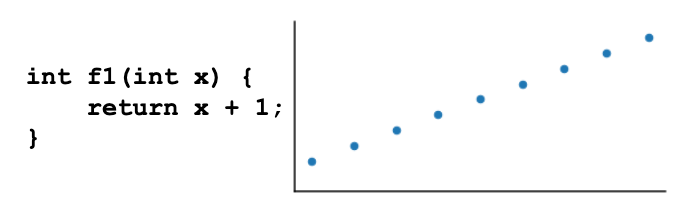
\includegraphics[width=\textwidth]{figs/f1}
  \end{subfigure}
  \begin{subfigure}[b]{0.32\linewidth}
    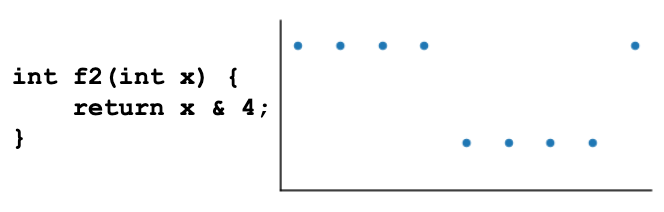
\includegraphics[width=\linewidth]{figs/f2}
  \end{subfigure}
  \begin{subfigure}[b]{0.32\linewidth}
    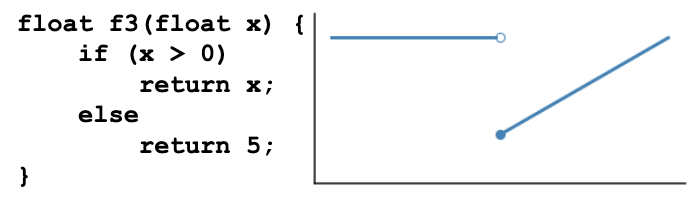
\includegraphics[width=\linewidth]{figs/f3}
  \end{subfigure}
  \vspace{-10pt}
   \caption{ Types of discrete and nonsmooth operations that occur in programs. \tc{f1} is a linear function that is still not differentiable because it operates on integers, while \tc{f2} performs bitwise \tc{and}, which is both discrete and nonsmooth. \tc{f3} illustrates a discontinuity due to branching and merging.}
  \label{fig:ex_funcs}
  \vspace{-10pt}
\end{figure*}

\subsection{Nonsmooth Gradient Approximation}

Programs are inherently difficult to differentiate because their behavior is generally discrete and nonsmooth, meaning that they cannot be differentiated directly. This behavior comes primarily from branches and memory operations, but also from many discrete operations such bitwise operators and integer arithmetic. Figure ~\ref{fig:ex_funcs} gives three examples of different types of operations that are difficult to differentiate. \tc{f1} is a simple linear function, but still is not analytically differentiablebecause it operates on integers and is discrete. \tc{f2} is also discrete, but introduces additional nonsmoothness with a \tc{and} operation. \tc{f3} shows how even on floating point operations branching can result in nonsmooth behavior.

Fortunately, extensive work has been done in the field of optimization on methods for approximating gradients over discrete and nonsmooth functions. The type of approximation that used depends on whether the function is convex, meaning that any point on the function can be connected to any other point by a straight line without going 'under' the function. Operations like addition and multiplication, or multiplying a variable by itself, are convex, but bitwise operations and discontinuities from branching generally are not. When the functions being analyzed are convex, a type of gradient approximation called subgradients may be used that behave similarly to gradients on smooth functions with regard to composition and global convergence properties. When functions are nonconvex, an extension of subgradients called generalized gradients may be used that allow optimization to still be performed, although they relax the composition and convergence properties of subgradients ~\cite{clarke1990optimization, rockafellar2009variational}.

\begin{figure}
  \centering
  \begin{subfigure}[b]{0.48\columnwidth}
    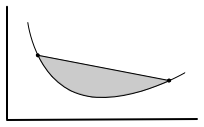
\includegraphics[width=\linewidth]{figs/convex_example}
    \caption{\label{fig:convex_ex} Convex function. Any line between two points on the function will pass 'over' the function.}
  \end{subfigure}
  \hspace{0.15cm}
  \begin{subfigure}[b]{0.48\columnwidth}
    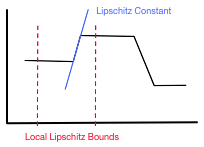
\includegraphics[width=\linewidth]{figs/lipschitz_ex}
  \caption{\label{fig:lipschitz_ex} Function with local Lipschitz Constant.}
  \end{subfigure}
  \vspace{-10pt}
  \caption{\label{fig:convex_lip_ex} Subgradient and Generalized Derivative examples.}
  \vspace{-15pt}
\end{figure}

\noindent \textbf{Convex Gradient Approximation.} Subgradients have been used in these cases to successfully optimize a wide variety of nonsmooth problems when the functions involved were convex ~\cite{beck2017first}. Subgradients are defined to be any vector under a convex function that intersects the function at the point the subgradient is evaluated, or formally, a vector $v$ is a subgradient of a function $f$ at a point $\bar{x}$ if:

\vspace{-10pt}\begin{align}
  f\left(x\right) \geq f\left(\bar{x}\right) + \langle v, x-\bar{x} \rangle \textrm{ for all } x \in \textrm{dom}\left(f\right)
\end{align}

This definition means that any point on the subgradient vector $v$ ($\langle v, x-\bar{x}$) for which $f$ is defined ($x \in \textrm{dom}\left(f\right)$), the value of the subgradient starting from the point it touches the function $f$ can continue to touch $f$ but can never be greater than $f$. This means that there can actually multiple subgradients for a given point of a discrete convex function, as in the example in figure \ref{fig:subgradient}. It is important to note that subgradients can also be defined in terms of being greater than the function in the case one wants to find the highest values of $f$, but conventionally used with vectors under the surface of a function. 

Subgradients are valid for discrete functions and thus can be computed on integer operations like \tc{f1} in figure \ref{fig:ex_funcs}. The chain rule also applies to them, meaning that subgradients of several sequential operations can be multiplied together to give a valid subgradient for combined operations.

\noindent \textbf{Nonconvex Gradient Approximation.} Nonconvex operations (which have multiple minima and maxima) like \tc{and} in \tc{f2} of Figure \ref{fig:ex_funcs}, have points for which there is no valid subgradient. To address these cases, generalized gradients are used to approximate gradients over nonconvex functions. Generalized gradients are composed of generalized directional derivatives, which work like subgradients, but only 'look' in single direction, starting at the point where they are evaluated and remaining under the function. This allows generalized directional derivatives to be taken at points where there is no valid subgradient, as can be seen in figure \ref{fig:dir_deriv}.



%\begin{figure}
  %\centering
  %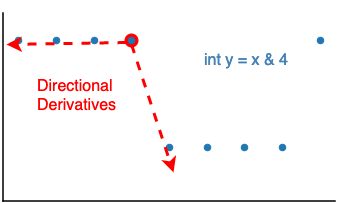
\includegraphics[width=0.7\columnwidth]{figs/directional_deriv_example}
  %\caption{\label{fig:dir_deriv} Directional derivative applied to a nonconvex function \tc{x \& 4}.}
%\end{figure}

We denote a generalized directional derivative in a directon $v$ as $f^\circ \left(x;v\right)$, which is formally defined as follows:

\vspace{-10pt}\begin{align}
  f^\circ \left(\bar{x}; v\right) = \lim \sup_{x \rightarrow \bar{x}, \lambda \downarrow 0} \frac{f\left(x + \lambda v\right) - f\left(x\right)}{\lambda}
\end{align}

\noindent Here $\bar{x}$ is the point at which the directional derivative is evaluated, $x$ can be any other point in the domain of $f$, and $\lambda$ is a distance along the vector $v$ that the derivative is taken in. The $\lim \sup_{x \rightarrow \bar{x}}$ notation indicates that the directional deriviative takes on the largest possible value for the two points $x$ and $x+\lambda v$ closest to $\bar{x}$ in the function's domain. The generalized gradient at a given point is then the set of all generalized directional derivatives for all possible directions from that point.

\begin{figure}
  \centering
  \begin{subfigure}[b]{0.45\columnwidth}
    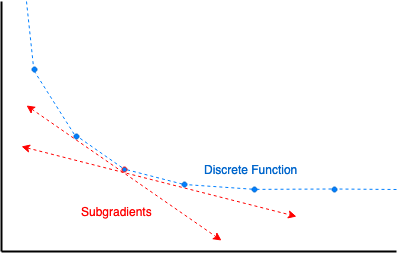
\includegraphics[width=\linewidth]{figs/subgradient_example}
    \caption{\label{fig:subgradient} Example of subgradient on discrete nonsmooth function.}
  \end{subfigure}
  \hspace{0.15cm}
  \begin{subfigure}[b]{0.5\columnwidth}
    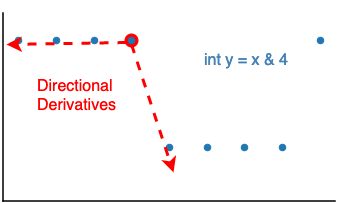
\includegraphics[width=\linewidth]{figs/directional_deriv_example}
  \caption{\label{fig:dir_deriv} Directional derivative applied to a nonconvex function \tc{x \& 4}.}
  \end{subfigure}
  \vspace{-10pt}
  \caption{\label{fig:grad_exs} Subgradient and Generalized Derivative examples.}
  \vspace{-15pt}
\end{figure}

\noindent \textbf{Lipschitz Continuity.} One important requirement of subgradients and generalized gradients is that the gradients of the functions they are computed over must be bounded. This property is called 'Lipschitz Continuity', and is defined as

\vspace{-10pt}\begin{align}
  |f\left(x_1\right) - f\left(x_0\right)| \leq K|x_1 - x_0|\\
  \textrm{ for all } x_1, x_0 \in x+\eta B \nonumber
\end{align}

\noindent where $K$, the Lipschitz Constant, is the bound on the gradient and $B$ denotes the size of the region in the domain of $f$ where the property is defined. Fortunately for the purpose of modeling programs, all operations ultimately occur on fixed width data types, limiting the range of values they can take on to the minimum and maximum of these data types and making them Lipschitz Continuous even in the worse case where a function jumps between extreme values.


\noindent \textbf{Proximal Gradients.} Subgradients and generalized gradients are useful guides analysis of discrete and nonconvex functions, but cannot be evaluated on general functions without sampling every possible value, which obviously isn't practical. To make evaluation tractable, we borrow another gradient approximation method from the discrete optimization literature called proximal gradients ~\cite{parikh2014proximal}. Instead of combining every possible surface or supporting vector under a function like subgradients and generalized gradients, proximal gradients use the minimum point within a soft bounded region. This region is defined by a cost function that increases quadratically with distance from the evaluation point. 

By representing the gradient with a single value and bounding the region in which it is evaluated, the proximal gradient makes the general problem of evaluating gradients tractable. The proximal operator is defined as follows when evaluated on a given point $\bar{x}$:

\vspace{-10pt}\begin{align}
  prox_f\left(\bar{x}\right) &= argmin_x \left(f\left(x\right) + \tfrac{1}{2}|| x-\bar{x}||_2^2\right)
\end{align}

The notation $argmin_x$ indicates that the operator selects the value of $x$ that minimizes both value of function $f\left(x\right)$ and the distance cost $\left(\tfrac{1}{2}\right)|| x-\bar{x}||_2^2$ that increases quadratically with the distance of $x$ from $\bar{x}$. Evaluating the proximal operator will give the minimum point near the point at which it is evaluated. This point can then be used to compute the largest directional derivative in the region near the point. 

% PROXIMAL GRADIENT
\vspace{-10pt}\begin{align}
  prox_{\nabla f}\left(\bar{x}\right) &= \frac{f\left(\bar{x}\right) - f\left(prox_f\left(\bar{x}\right)\right)}{\bar{x} - prox_f\left(\bar{x}\right)}
\end{align}

\noindent \textbf{Sampling Bounds.} On functions that are Lipschitz Continuous, the region that must be sampled to evaluate the proximal operator can be hard bounded as a factor of the Lipschitz Constant $K$. This bound is derived by observing that the cost function of the proximal operator is upper bounded by the initial function value and lower bounded by linear function decreasing at rate $K$ from the point $\bar{x}$ for $prox_f(\bar{x})$.

% BOUNDS DERIVATION 1
\vspace{-10pt}\begin{align*}
  \left(f\left(\bar{x}\right) - K*||prox_f\left(\bar{x}\right) - \bar{x}||_2  + \tfrac{1}{2}|| prox_f\left(\bar{x}\right)-\bar{x}||_2^2\right)\\
    \leq \left(f\left(prox_f\left(\bar{x}\right)\right) + \tfrac{1}{2}|| prox_f\left(\bar{x}\right)-\bar{x}||_2^2\right)\\
    \leq f\left(\bar{x}\right) + \tfrac{1}{2}||\bar{x} - \bar{x}||_2^2
\end{align*}

Here the term $f\left(\bar{x}\right) - K*||prox_f\left(\bar{x}\right)$ represents the minimum value $f$, can take as $prox_f\left(\bar{x}\right)$ moves farther from $\bar{x}$ due to its Lipschitz Constant $K$, while the value $f\left(\bar{x}\right) + \tfrac{1}{2}||\bar{x} - \bar{x}||_2^2$ represents the value being minimized at the initial point $\bar{x}$. This can be simplified by dropping the middle term: 

\vspace{-10pt}\begin{align*}
  \left(f(\bar{x}) - K*||prox_f\left(\bar{x}\right) - \bar{x}||_2  + \tfrac{1}{2}|| prox_f\left(\bar{x}\right)-\bar{x}||_2^2\right)\\
    \leq f\left(\bar{x}\right)
\end{align*}


as well as subtracting $f\left(\bar{x}\right)$ from both sides:

\vspace{-10pt}\begin{align*}
  \left( - K*||prox_f\left(\bar{x}\right) - \bar{x}||_2  + \tfrac{1}{2}|| prox_f\left(\bar{x}\right)-\bar{x}||_2^2\right) &\leq 0
\end{align*}

Adding $K*||\bar{x}-x||_2$ to both sides, dividing by $||\bar{x}-x||$, and multiplying by 2 gives a bound of $2K$ on the distance between the inital point $\bar{x}$ and the proximal operator result $prox_f\left(\bar{x}\right)$. 


\vspace{-10pt}\begin{align}
    || prox_f(\bar{x})-\bar{x}||_2 &\leq 2K
\end{align}

This means that the distance the result of the proximal operator from its initial $\bar{x}$ is bounded by at most twice the Lipschitz Constant for the function, $2K$. In practice a scaling factor $\lambda$ is often used with the proximal operator to adjust the relative weighting of distance from the evaluation point. When the scaling factor is added the bound becomes $2 \lambda K$. We then denote the Proximal Operator with a Lipschitz sampling bound $K$ and scaling factor $\lambda$ as

\vspace{-10pt}\begin{align}
  prox_f\left(\bar{x}, K, \lambda\right) &= argmin_x \left(f\left(x\right) + \tfrac{1}{2\lambda}|| x-\bar{x}||_2^2\right) \nonumber\\
  \textrm{s.t. } &|| x-\bar{x}||_2 \leq 2 \lambda K
\end{align}

\noindent and the associated bounded Proximal Gradient is:

\vspace{-10pt}\begin{align}
prox_{\nabla f}\left(\bar{x}, K, \lambda\right) &= \frac{f\left(\bar{x}\right) - f\left(prox_f\left(\bar{x}, K, \lambda\right)\right)}{\bar{x} - prox_f\left(\bar{x}, K, \lambda\right)}
\end{align}

This provides theoretically sound and adjustable method for bounding the sampling region on Lipschitz Continuous functions when the Lipschitz Constant $K$ is known.


\gabe{Probably should also explain smoothing here}

\subsection{Automatic Gradient Computation}

Automatically computing gradients over programs composed of analytically differentiable operations is a process called Automatic Differentiation, or 'AutoDiff', that has been a longstanding tool in computational modeling and is a core component of deep learning frameworks such as Tensorflow ~\cite{Wengert:1964:SAD:355586.364791, tensorflow2015-whitepaper}. Autodiff makes use of the chain rule in calculus to compute the gradient over a program as a series of gradients of individual operations multiplied together, each of which can be computed analytically. However, AutoDiff methods and frameworks have traditionally limited themselves to working with  functions that are at minimum piecewise differentiable, and do not support nonsmooth operations found in general programs such as bitwise operations or merge operations. By leveraging proximal gradients, the Autodiff approach can be extended to work with nonsmooth operations as well, thereby making it possible to compute gradients over general programs.





%-------------------------------------------------------------------------------
\section{Working Example}
%-------------------------------------------------------------------------------

\begin{figure}
  \centering
  \begin{subfigure}[b]{0.48\columnwidth}
    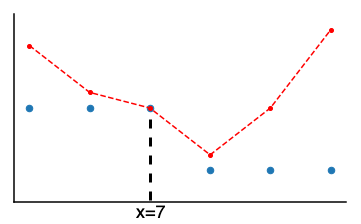
\includegraphics[width=\linewidth]{figs/sosp-working_ex3}
    \caption{\label{fig:working_ex1}Proximal cost function at $\bar{x} = 7$.}
  \end{subfigure}
  \hspace{0.1cm}
  \begin{subfigure}[b]{0.48\columnwidth}
    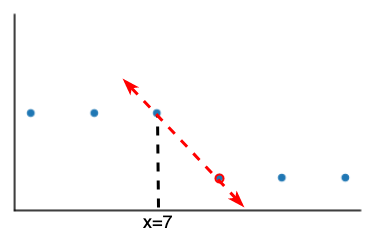
\includegraphics[width=\linewidth]{figs/sosp-working_ex2}
    \caption{\label{fig:working_ex2}Evaluated Proximal Gradient for $\bar{x} = 7$.}
  \end{subfigure}
  \vspace{-15pt}
  \caption{\label{fig:working_ex}Example of Proximal Gradient Evaluation.}
  \vspace{-15pt}
\end{figure}

To give a better intuition for how proximal gradients work in practice, we provide a working example. Consider the function $f(x) =   x \texttt{\&} 4$ shown in figure \ref{fig:ex_funcs}, and suppose we are evaluating it with $\bar{x} = 7$. This type of bitwise operation is common in programs that parse a file for input, since they frequently need to check if flag bits are set in a header or section header of the file. However, discrete functions like bitwise operations are nondifferentiable so we instead evaluate the proximal gradient.

To evaluate the proximal gradient on $f\left(x\right)$, the sampling region must first be defined. \tc{x \& 4} has a Lipschitz Constant of $K=4$ (any bitwise operation with a constant has a Lipschitz Constant with the value of the most significant bit in the constant), so assuming a proximal scaling factor of $\lambda = 1$, the sampling distance bound is $2K = 8$. Therefore, a total of 16 samples must be taken, for $x = [-1, 15]$, and the cost function of the proximal operator, $f(x) + ||x - \bar{x}||_2^2$ evaluated for each possible $x$. Figure \ref{fig:working_ex1} shows the value of the cost function near $x = 7$, there is a clear minimum at $x=8$, where $f\left(8\right) + ||8-7||_2^2 = 1$, so the proximal operator evaluates to $x=8$. The proximal gradient is then $prox_{\nabla f}\left(7\right) = \frac{f\left(7\right) - f\left(8\right)}{7 - 8} = -4$.




%-------------------------------------------------------------------------------
\section{Gradient Analysis Framework}
%-------------------------------------------------------------------------------

The gradient analysis framework works similarly to autodifferentiation, computing the gradient of each operation and using the results as inputs to the next gradient. However, unlike autodifferentiation, nonsmooth functions are handled by Proximal Gradients, so that a meaningful gradient can be computed over all program operations. Since Proximal Gradients require local Lipschitz Constants to bound their sampling in some cases, Lipschitz Constants are also propogated over the program along with the gradient.

\noindent \textbf{Gradient Propogation with Chain Rule.} We model a program as an arbitrary function $P$, that operates on the system state $x$ and produces a modified system state $x'$. Since programs are generally nonsmooth, we can use subgradients to approximate the gradient of $P$. Programs in general are too complex to model, but since the program $P$ is composed of individual operations whose behavior is known, we model $P$ as a composition of $N$ individual functions on the system state that represent each operation in the program:

\vspace{-10pt}\begin{align*}
P(x) = P_N \circ P_{N-1} \circ \cdots \circ P_2 \circ P_1 (x)
\end{align*}

Subgradients compose under the chain rule, so we apply the same approach used in Automatic Differentation to evaluate the subgradient of $P$,  $\nabla_{sub} P(x)$ by computing the product of the subgradients of each operation in $P$ ~\cite{rockafellar2009variational}. 

\vspace{-10pt}\begin{align*}
  \nabla_{sub} P(x) = \nabla_{sub} P_N * \nabla_{sub} P_{N-1} * \cdots * \nabla_{sub} P_2 * \nabla_{sub} P_1
\end{align*}

This is the same approach used in Automatic Differentiation, but applied to discrete functions and subgradients instead of continuous functions with gradients. Then, instead of attempting to evaluate a subgradient over the program function $P$, which has unknown behavior and operate on a large number of variables, subgradients can be evaluated on the individual operations $P_i$, which have known behavior and usually only operate on 1 or 2 variables.

For some operations that are analytically differentiable on continuous variables, the subgradient of the operation on discrete variables can also be computed analytically. However, the subgradients of nonsmooth operations must be approximated with Proximal Gradients. 

\noindent \textbf{Sampling Bounds with Lipschitz Constants.} In order to bound the samples required to evaluate the Proximal Gradient, Lipschitz Bounds must also be known for each operation. Fortunately, Lipschitz Bounds can be computed for each type of nonsmooth operation in a program based on its behavior and the Lipschitz bounds of its input. This means that in addition to propogating the gradient through a program, we also compute the Lipschitz Constant on each operation based on the Lipschitz Constants of its inputs, and propogate the result to the next function.

In some cases the Lipschitz Constant $K_f$ cannot be derived from knowledge of the function, so it is estimated by sampling the function at $x \pm K$ and taking the maximum difference.

\noindent \textbf{Partial Derivatives.} A gradient is composed of partial derivatives with regard to each part of the input, so when defining rules for computing the gradient we focus on partial derivatives with regard to the variable in the system state that was first marked for tracking, which is denoted $x_i$. Typically $x_i$ is a byte in an input read from a file or socket, but may also be an internal program variable.


\noindent \textbf{Program Inputs.} In the case where $g$ and $h$ are direct inputs to the program, such as bytes read from a file, we consider them to be identity functions with a partial derivative of 1 if they operate on the byte of the input that the partial derivative is being taken with regard to, and 0 otherwise. The Lipschitz Constant in this case is also 1.

\noindent \textbf{Propogation rules.} We then define gradient and Lipschitz Constant propogation rules as follows, where $f$ represents the current operation and $g$ and $h$ represent the prior operations on its input.

\begin{enumerate}
  \item \textbf{Addition and Multiplication.} Addition and multiplication, as well as subtraction, are examples of discrete functions whose subgradients can still be computed analytically and therefore do not require sampling. The partial derivatives and associated Lipschitz Constants with regard to the $i$th input variable $x_i$ can then be computed as follows based on the definition of $f$ as $f\left(g, h\right) = g+h$:

\vspace{-10pt}\begin{align*}
  K_f &= K_{g} + K_{h} &\tfrac{df}{dx_i} &= \tfrac{dg}{dx_i} + \tfrac{dh}{dx_i}
\end{align*}

Multiplication can likewise rely on analytical derivatives as it is a linear operation:

\vspace{-10pt}\begin{align*}
  K_f &= h*K_{g} + g*K_{h} & \frac{df}{dx_i} &= h\frac{dg}{dx_i} + g\frac{dh}{dx_i}
\end{align*}

    \gabe{These are pretty obvious, textual description may be sufficient.}


\item \textbf{Integer Division.} Unlike division with continuous values, division on integers is not a linear function because any fractional portion of the result is truncated. Therefore sampling the function is necessary to evaluate an accurate partial derivative. To compute the Lipschitz Constant, we use the quotient rule and consider the case that causes the maximum possible change in $f$, where $\tfrac{dg}{dx_i} = K_g$, and $\tfrac{dh}{dx_i} = -K_h$.

\vspace{-10pt}\begin{align*}
  K_f &= \frac{K_g h + K_h g}{h^2} & 
  \frac{df}{dxi} &= prox_{\nabla f}\left(\bar{x}, K_f, \lambda\right)
\end{align*}

\item \textbf{Modulo Operations.} Like integer division, modulo operations are also generally nonsmooth and require evaluating the proximal gradient. In cases the modulo operand is constant, which we found usually the case in our test programs, the Lipschitz Constant for the modulo function is simply the modulo operand:

\vspace{-10pt}\begin{align*}
  K_f &= h &
  \frac{df}{dxi} = prox_{\nabla f}\left(\bar{x}, K_f, \lambda\right)
\end{align*}

In cases where the derivative of the modulo operand is nonzero, the Lipschitz Constant is estimated by sampling and used to evaluate the Proximal Gradient. 


\item \textbf{Shift Operations.} Shift operations can be defined as a multiplication with an exponent, but have the additional condition that bits shifted past the width of the datatype are dropped. Therefore the Lipschitz Constant is also estimated by sampling and used to evaluate the Proximal Gradient.


  \gabe{May want to combine integer division, modulo and shift.}

\item \textbf{Bitwise Operations.} When one of the operands of a bitwise operation is a constant, or at least has a 0 derivative with regard the marked input, the Lipschitz Constant can be set the value of the highest set bit in the constant operand. However, in cases where both operands have nonzero derivatives, the Lipschitz Constant must be estimated and used to evaluate the Proximal Gradient. 


\item \textbf{Memory Indexing.} Indexing into an array in memory can be modeled as an arbitrary nonsmooth function $f\left(g\right)$. Since we cannot derive the Lipschitz Constant $K_f$ from knowledge of the function, we estimate it by sampling the function at $g \pm g'$ and taking the maximum difference. The proximal gradient can be computed using the estimated Lipschitz Constant

%\begin{align*}
  %f\left(g\right) &= \textrm{mem}\left[g\right]\\
  %\frac{df}{dxi} &= prox_{\nabla f}\left(\bar{x}, K_f, \lambda\right)
%\end{align*}

\item \textbf{Load Operations.} Load operations will normally take on the saved partial derivative of whatever variable was originally saved to that memory location. However, there is possibility that one or more types with smaller bit widths are being loaded into a single larger width type. In these cases each partial derivative and Lipschitz Constant associated with an address being loaded, if there are more than one, is shifted by its offset with the base address and summed with the others.

\vspace{-10pt}\begin{align*}
  K_f &= \sum_j K_j 2^{offset_j} &
  \frac{df}{dxi} &= \sum_j \frac{d \textrm{addr}_j}{dx_i}2^{offset_j}
\end{align*}


\item \textbf{Integer Branches.} In cases where a variable can take on different values based on which portion of the branch was executed, we model the branch and subsequent merge as either a piecewise point function or a piecewise step function, depending on if the branch comparison defines a single value or set of values, such as greater than. In order to the Proximal Gradient on this function, the alternate branch path must be sampled to determine its value in the merge operation. In practice any execution of an alternate path will be invalid, but for many branches will still result in an accurate representation of program behavior. In cases where the sample execution does not return to the merge operator, the alternate branch portion of the piecewise function is considered to be undefined, resulting in a partial deriviative of 0. Once the path has been sampled, the Proximal Gradient can be evaluated on it normally, and the associated Lipschitz Constant can be set to the size of the step in the piecewise function.

  This approach will handle most single branches, but breaks down in the case where multiple nested branches on different values must be bypassed for the merge variable to be set. To handle these cases, when sampling alternate branch paths any subsequent branch encountered can also be sampled, and the Proximal Gradient computed over each branch individually. Figure \ref{fig:branch_exs} shows how this process works on nested branches with two conditions, \tc{x>1} and \tc{set>0}. When the branch is initially executed with \tc{x=0} and \tc{set=0}, the result is \tc{y=0}. To evaluate Proximal Gradient, the first branch is sampled by executing the alternate path with \tc{x=2}. This execution also results in \tc{y=0}, but during it the second nested branch on \tc{set} is encountered and sampled with \tc{set=1}, which results in \tc{y=1}. These samples are then used to form a function that is 1 for \tc{x>1} and \tc{set>0} and 0 elsewhere. The closest point to \tc{x=0, set=0} that gives the greatest change on this function is \tc{x=2, set=1}, so the Proximal Gradient evaluates on that point, resulting in partial derivatives of $\tfrac{dy}{dx}=\tfrac{1}{2}$ and $\tfrac{dy}{dset} = 1$.

\begin{figure}
  %\centering
  \begin{subfigure}{0.38\columnwidth}
    %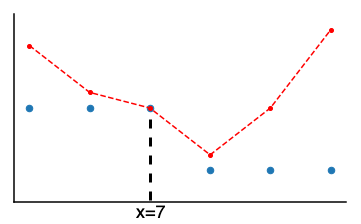
\includegraphics[width=\linewidth]{figs/sosp-working_ex3}
    \begin{lstlisting}
// int x=0 
// bool set=0
int y=0;
if (x>1)
    if (set==1)
        y=1;
    \end{lstlisting}
    %\caption{\label{fig:branch_ex1}Example of nested branch with $\tfrac{dy}{dx}=\tfrac{1}{2}$ and $\tfrac{dy}{dset} = 1$}
  \end{subfigure}
  \hspace{0.1cm}
  \begin{subfigure}{0.58\columnwidth}
    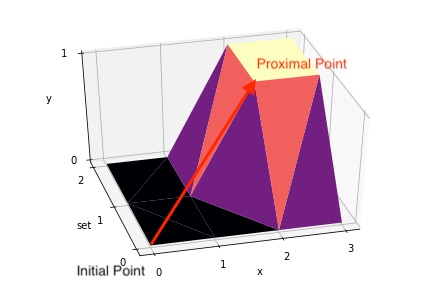
\includegraphics[width=\textwidth]{figs/nested_branch_plot.jpg}
    %\caption{\label{fig:branch_ex2}Surface}
  \end{subfigure}
  \vspace{-0pt}
  \caption{\label{fig:branch_exs}Example of nested branch with $\tfrac{dy}{dx}=\tfrac{1}{2}$ and $\tfrac{dy}{dset} = 1$.}
  \vspace{-0pt}
\end{figure}


\item \textbf{Floating Point Branches.} Unlike derivatives of integer operations, derivatives of floating point operations can generally be computed analytically, as is done in existing autodifferentiation frameworks. The exception to this is branches, which are normally not handled. Like integer branches, we model branches with floating point values as a piecewise step function, and execute the alternate branch path to determine the value of the step. However, unlike integer branches, floating point branches are not locally lipschitz, because they have an infinite slope at the point of discontinuity \gabe{add a figure showing this}, so a Proximal Gradient cannot be evaluated on them. Instead, we apply a Gaussian smoothing function, where the variance of the gaussian used is set according the magnitude of the input derivative.
\end{enumerate}




%-------------------------------------------------------------------------------
\section{Implementation}
%-------------------------------------------------------------------------------

We implemented Proximal Gradient Analysis as a new type of code sanitizer in the LLVM Framework. LLVM is a compiler framework that uses an Intermediate Representation that resembles high level assembly for instrumentation and optimization ~\cite{llvm2004}. LLVM sanitizers are specialized LLVM passes that add instrumentation to code intended to help detect undesirable behavior and 'sanitize' it. Adding instrumentation at the IR level allows it to be compiled into the binary, making it significantly faster than instrumenting the binary directly, and allowing it to operate on programs written in any language supported by LLVM.

Our implementation is based on the dynamic taint tracking sanitizer in LLVM, known as DataFlowSanitizer or dfsan. DataFlowSanitizer uses shadow memory to track taint labels. For each byte of application memory, there are two corresponding bytes of shadow memory that store the taint label for that byte. Therefore there can be up to $65,536$, or $2^{16}$, unique labels. Metadata associated with each label is stored in an array that is indexed by the labels. New labels representing a union of current labels are generated whenever an operation has multiple labeled inputs, and these unions are tracked in a seperate  table.

We made the following modifications to the DataFlowSanitizer architecture in order support gradient analysis. First, we added additional metadata for each label representing positive and negative directional derivatives for the current marked byte. Second, we eliminated the union table and modified the instruction visitors to generate a new label and compute derivatives for that label if any of the inputs are labeled.  This results in the generation of more labels, as every differentiable operation with a labeled input creates a new label, but is necessary since each operation will have unique derivatives for a given set of inputs. 

Figure \ref{fig:grsan_diagram} illustrates how this architecture works for a single instrumented operation. First a new label is generated for the variable \tc{y}, and assigned to the corresponding 16 bit location in the shadow memory. The derivative of \tc{x*2} is then computed and stored in the derivative table at the index of the new label.

\begin{figure}
    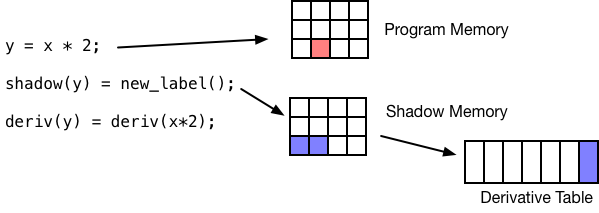
\includegraphics[width=\columnwidth]{figs/grsan_layout}
  \vspace{-20pt}
  \caption{\label{fig:grsan_diagram}Gradient Sanitizer architecture.}
  \vspace{-10pt}
\end{figure}

LLVM has a total of 66 instructions, but the majority of these involve control flow and data movement that can either be left uninstrumented or handled by copying or setting shadow memory. Operations that only require simple manipulations of shadow memory are handled by adding LLVM instrumentation directly to the program. For more complex operations, we inject calls to a dynamically linked library that implements the gradient computation and tracking.

\noindent \textbf{Binary Operations} Most of the differentiable instrucitons in LLVM are binary operators, of which there are 18, 5 floating point and 13 integer. The integer operations include both signed and unsigned versions, as well as bitwise operations. Specific gradient instrumentation functions for 8, 16, 32, and 64 bit integer functions are defined, as well as floats and doubles. Since LLVM does not distinguish between signed and unsigned in its types, all integer derivative functions take the unsigned value of the operation arguments as parameters and perform an unchecked cast to the signed type if the operation is signed. Figure \ref{fig:binop_code} shows an excerpt of the derivative instrumenation for a 32 bit integer. The function first checks the input labels and exits if neither input is labeled. If at least one input is labeled, the instrumentation aquires a new label and looks up derivatives for its labeled inputs. It then computes derivatives for the instruction based on the input derivatives and stores them in the global label information table. Finally it returns the new label, which will be saved to the shadow address associated with the instruction.

\noindent \textbf{Memory Operations} LLVM has 3 instructions involving memory that require special handling: Alloca, Load, Store. The Alloca instruction allocates space on the stack for a variable, so during instrumentation an additional allocation is added to track the associated shadow, and an associative list of the shadows of current stack variables is maintained for reference. This allows operations on stack variable shadows to be performed directly without adding extra lookups to shadow memory at runtime. Loads are implemented as specified in the methodology section, if the shadow for the loaded memory contains multiple labels, the derivatives of those labels are shifted by multiplied by their offset and added together. For Store instructions the shadow of the variable being stored is first looked up, which may be a stack variable or involve adding a shadow memory lookup, and then written to the shadow of the address the variable is being written to.

\noindent \textbf{Indexing Operations} LLVM has two instructions that represent memory indexing, the GetElementPtr and ExtractValue instructions. GetElementPtr performs pointer arithmetic to return a pointer to a specified object and offset, while ExtractValue returns a concrete value. In both cases we compute derivatives by sampling based on the input derivative. \gabe{Have not implemented this yet, add details once we implement it.}

\noindent \textbf{Type Operations} There are 13 instructions related to type casting in LLVM. Most of these can be safely handled by simply copying labels from the original value to the result, but instructions for value truncation, and conversions from floating point to integer, require sampling. \gabe{Right now we don't handle these but should probably add them for completeness.}

\noindent \textbf{External Function Calls} Generally the return function calls to uninstrumented code are left unlabeled, but some operations in glibc are given instrumentation. Labels for any buffer overwritten by fread or memset are set to 0, and labels for buffers copied by memcpy or strcpy are likewise copied. LLVM also contains intrinsic functions for copying and allocating memory that are handled similarly. 

%- External Function calls
%- We refer to our implementation as GradientSanitizer, or grsan. The Gradient Saniziter is composed of two components, the Sanitzer that checks each LLVM operation and determines what instrumentation to add to perform the gradient analysis, and a dynamically linked library that implements the gradient analysis itself.\gabe{Put diagram here source code -> clang -> LLVM IR -> grsan -> LLVM backend -> binary -- linked grsan instrumentation} \\
%- explain shadow memory and labels\\

%\noindent \textbf{Sanitizer Component}\\
%- the sanitizer componenent implements the LLVM visitor pattern, which visits each operation in a program and and allows the user to change it or add custom instrumentation.\\
%- LLVM has a total of X operations. For many of them we simply propogate labels. For some we calculate gradients \gabe{put in table with LLVM ops and handling}\\
%- when a value is allocated on the stack, 

%\noindent \textbf{Gradient Instrumentation}\\
%- Generally the Gradient Instrumentation operates as follows:\\
%- most operations such as load and stores

\begin{figure}
\begin{lstlisting}
uint16_t grsan_union_int(uint16_t l1, uint16_t l2, 
                         uint32_t x1, uint32_t x2, 
                         uint16_t opcode) { 
  float neg_dx1 = 0, neg_dx2 = 0, 
        pos_dx1 = 0, pos_dx2 = 0, 
        neg_dydx, pos_dydx; 
  if (l1 == 0 && l2 == 0) { 
    return 0; // exit early if unlabeled
  } 
  grsan_label label = 
                atomic_fetch_add(&__grsan_last_label, 1, 
                              memory_order_relaxed) + 1; 
  if (l1 != 0) { 
    neg_dx1 = __grsan_label_info[l1].neg_dydx;
    pos_dx1 = __grsan_label_info[l1].pos_dydx;
  }
  if (l2 != 0) {
    neg_dx2 = __grsan_label_info[l2].neg_dydx;
    pos_dx2 = __grsan_label_info[l2].pos_dydx;
  }
  switch (opcode) { 
    case 15: // opcode 15 = llvm integer multiplication
      neg_dydx = x1 * neg_dx2 + x2 * neg_dx1;
      pos_dydx = x1 * pos_dx2 + x2 * pos_dx1;
      break;
    case 26: {  // opcode 26 = llvm bitwise And
      uint32_t y = x1 & x2;
      uint32_t neg_y = (x1 - uint32_t(neg_dx1)) 
                          & (x2 - uint32_t(neg_dx2));
      neg_dydx = y - neg_y;
      uint32_t pos_y = (x1 + uint32_t(pos_dx1)) 
                          & (x2 + uint32_t(pos_dx2));
      pos_dydx = pos_y - y;
      break;
    }
    // ...more operations...
    // default to nan derivatives for unexpected opcode
  }
  __grsan_label_info[label] = (struct grsan_label_info) 
        { l1, l2, opcode, neg_dydx, pos_dydx };
  return label;
}
\end{lstlisting}
  \caption{\label{fig:binop_code}Sample of gradient compution with both analytic integer multiplication and sampling bitwise \tc{And} examples.}
\end{figure}






%-------------------------------------------------------------------------------
\section{Evaluation}
%-------------------------------------------------------------------------------

We evaluate Gradient Analysis both by comparing it with taint as a method of dataflow analysis, and in direct applications for vulnerability detection. Specifically, we run experiments to answer the following questions:

\begin{itemize}
  \item Does gradient analysis add more overhead than taint analysis?
  \item Is gradient analysis more accurate than taint analysis in predicting dataflows?
  \item Does using gradient analysis to guide fuzzing lead to better coverage?
  \item Can gradient analysis detect recent CVEs that taint is typically used to detect?
  \item Is gradient analysis an effective tool for vulnerability discovery?
\end{itemize}

\subsection{Test Programs}

We perform tests on a set 5 widely used file parsing libraries and 7 total programs. We select these programs to cover most common file types that must be routinely parsed and rendered from untrusted sources, and therefore are common vectors for attacks.

\begin{table}
\centering
 \begin{tabular}{ll l l} 
 \toprule
  Library & Test Program & SLOC & File Format \\ 
 \midrule
 zlib-1.2.11    & \verb|minigzip -d| & \gabe{TODO}    & GZ/ZIP \\ 
 mupdf-1.14.0   & \verb|mutool show| & 123,562    & PDF \\  
 libxml2-2.9.7  & \verb|xmllint| & 73,920    & XML \\
 libjpeg-9c     & \verb|djpeg| & 8,857    & JPEG \\
 %harfbuzz-1.7.6 & \verb|minigzip -d| &  9,853   & TTL \\
                & \verb|readelf -a| & 21,647    &  \\  
 binutils-2.30  & \verb|objdump -xD| & 72,955  & ELF \\  
                & \verb|strip | &  56,330   &  \\  
 \bottomrule
 \end{tabular}
  \caption{Summary of parser programs used in evaluation. \gabe{TODO compile with gcov to get linecounts  }}
  \label{tab:programs}
\end{table}


\subsection{Taint Tracking Comparison}

Since proximal gradient analysis is a new form of dynamic dataflow analysis, we focus most of our evaluation on comparisons with dynamic taint tracking, which is the most widely used version of dynamic dataflow analysis. For our comparison, we use the implementation of taint tracking in LLVM's DataFlowSanitizer. Since our implementation of proximal gradient analysis is based on the DataFlowSanitizer architecture, we ensure that differences in performance on evaluation tasks are due to the differences between gradient and taint as dataflow methods, and not any differences in the underlying frameworks or architecures used in their implementation. 

We compare proximal gradient analysis with taint tracking in three areas: first, we evaluate the overhead introduced by the dataflow tracking instrumentation. Second, we estimate the accuracy of the dataflows predicted by gradient and taint by perturbing input bytes. Third, we compare the coverage achieved by a fuzzer using gradient and taint predictions as a guide. 


\subsubsection{Performance Overhead}

We first address the question of how much overhead the instrumentation for gradient analysis adds to a program. To measure overhead, we first execute each program 50 times to ensure cache locality, and then execute 5000 times while recording runtime. Since individual executions of the test programs usually complete in less than a kernel tick (1 millisecond), we measure walltime instead of cpu time for all 5000 executions and compute mean runtime from that. We measure overhead for each program on a small input file, where the inputs range in size from 3.7Kb for JPEG to 8.5Kb for ELF. \gabe{can rerun with files of more similar size if needed.} The evaluation was performed on an Ubuntu 16.04 server with an Intel Xeon E5-2623 v4 2.60GHz CPU.

Table \ref{tab:performance} shows the results of the overhead comparison. \gabe{I feel like there are several things we need to sort out before discussing these results. In particular, some of the numbers are essentially identical for unlabeled vs labeled, and I'm not really sure why gradient is so much faster for libxml while slower for mupdf. Need to investigate which instructions are actually being processed to explain this intelligently. Also, may need to rerun with higher optimization than -O0 to see meaningful differences between labeled and unlabeled.}



\begin{table*}[t]
\begin{tabular}{@{}lllllllllll@{}}
\toprule
  & Base & \multicolumn{2}{c}{Unlabeled Taint} & \multicolumn{2}{c}{Unlabeled Gradient} & \multicolumn{2}{c}{Taint} & \multicolumn{2}{c}{Gradient} & Relative\\

  Program & Runtime & Runtime & Overhead & Runtime & Overhead & Runtime & Overhead & Runtime & Overhead & Overhead \\ 
\midrule
zlib & 0.00093 & 0.0015 & 0.56 & 0.0016 & 0.73 & 0.0015 & 0.57 & 0.0017 & 0.85 & 0.28 \\
jpeg & 0.00089 & 0.0014 & 0.59 & 0.0014 & 0.6 & 0.0015 & 0.63 & 0.0015 & 0.63 & -0.0017 \\
mupdf & 0.0031 & 0.0086 & 1.8 & 0.01 & 2.4 & 0.0086 & 1.8 & 0.01 & 2.4 & 0.59 \\
libxml & 0.0017 & 0.0072 & 3.2 & 0.0052 & 2.1 & 0.0072 & 3.2 & 0.0053 & 2.1 & -1.1 \\
readelf & 0.0012 & 0.0017 & 0.4 & 0.0017 & 0.41 & 0.0017 & 0.41 & 0.0018 & 0.46 & 0.046 \\
objdump & 0.0021 & 0.0021 & 0.017 & 0.0021 & 0.021 & 0.0021 & 0.016 & 0.0022 & 0.028 & 0.011 \\
strip & 0.0011 & 0.0022 & 0.95 & 0.0022 & 0.94 & 0.0022 & 0.96 & 0.0022 & 0.95 & -0.015\\ \bottomrule
\end{tabular}
 \label{tab:performance}
 \caption{Summary of performance. \gabe{Possibly add in ablation with label reuse optimization.}}
\end{table*}




\subsubsection{Dataflow Precision}

One of the main advantages gradient has over taint is that it naturally handles operations where numerical effects cause the input to have no effect on the output. These types of effects result in many situations where taint rules over approximate, marking large portions of the program as tainted when they are not and limiting the usefulness of taint as a tool for analysis. 

However, evaluating the extent to which overtainting occurs is difficult due to the exponential size of possible inputs. In theory, each possible input could be sampled to evaluate which input bytes can potentially effect a given internal program value and create a ground truth against which different dataflow methods could be evaluated. In practice complete evaluation is impossible so we sample a subset of possible inputs as follows: for each byte in the input that is predicted by taint, we generate sample inputs where the byte is set to 0, 255, and where each bit in the byte was toggled by 1 for a total of 10 samples per byte. We found that in practice this strategy usually resulted in a change to branch variables if it was possible to effect a change, since common patterns in branching were checking for 0, above or below a threshold, or if particular bits were set.

For our evaluation of precision we focus on branch constraints since these values most significantly effect the behavior of a program and are key to achieving good test coverage. Typically when dataflow is used in dynamic testing applications branch inputs are marked a sinks. \gabe{We could also mark a set of other functions if that makes sense.} For each branch input and each marked byte, we evaluate precision by recording its values over executions of all the input samples generated by modifying the byte. If any the modified inputs cause the branch value to change during execution, we consider that byte to have a valid dataflow to the branch input. 

We evaluate dataflow precision for taint and gradient on the parsing programs shown in table ~\ref{tab:programs} using a set of inputs generated by running afl on each program for an hour then running afl-cmin on the result. The results are shown in table (2) ~\ref{tab:precision_comp}. Gradient analysis is more precise than taint for all programs, although in some programs such as \tc{mutool} and \tc{xmllint} this improvement is relatively small. Overall, gradient is on average 32\% more precise than taint, as as much 42\% more precise for dataflow predictions on jpeg. We hypothesize that gradient gives a more significant improvement in accuracy when programs contain a large number of numerical operations, which often cause overtainting but are handled correctly by gradient. This effect can be seen in the large improvements for \tc{minigzip} and \tc{djpeg}, both of which use a large number of numerical operations to perform decompression on their inputs.

\gabe{TODO rerun this with recall recorded, calc f1, try to get higher coverage for readelf. Also would be nice to analyze what instructions are being instrumented here too and see how more sampling improves precision. Also add number of instrumented branches for each program, big numbers are impressive.}

\begin{table}
\centering
  \begin{tabular}{lrrr} 
 \toprule
    Test Program & Taint & Gradient & Relative \\ 
                 & Precision & Precision & Improvement \\ 
 \midrule
   minigzip (zlib-1.2.11)  & 0.593     & 0.917 & 0.324\\ 
   mutool (mupdf-1.14.0)   & 0.704     & 0.714 & 0.011\\
   xmllint (libxml2-2.9.7) & 0.957     & 0.988 & 0.032\\
   djpeg (libjpeg-9c)      & 0.519     & 0.942 & 0.423\\  
   readelf (binutils-2.30) & 0.074     & 0.075 & 0.001\\  
   objdump (binutils-2.30) & 0.352     & 0.516 & 0.163\\  
   strip   (binutils-2.30) & 0.344     & 0.585 & 0.241\\  
 \bottomrule
 \end{tabular}
 \caption{\label{tab:precision_comp}Summary of precision comparison results for taint and gradient Analysis.\abhi{need F1 score/recall}}
\end{table}



\subsubsection{Dataflow Guided Fuzzing}

Since dynamic dataflow analysis is often used as a tool to guide fuzzing, we next evaluate gradient analysis as a method for guided fuzzing. In order to perform a controlled comparison with taint tracking, we use the following procedure: first, the program under test is instrumented with dataflow method currently being tested, either gradient or taint, and modified to mark inputs when it processes a file. In addition, all of the programs branches are instrumented as sinks, so that dataflows to each branch from each input byte are recorded. The program is then executed on a single seed input, and the number branches each input byte has a dataflow to is recorded. The top 512 bytes are then selected based on the number of branches they effect, and targeted for fuzzing. 

To perform the fuzzing, we use a modified implementation of AFL that uses a strategy formulated for targeted important bytes. The fuzzer first targets each byte individually, and then doubles the number of bytes targeted in each subsequent search until it has targeted all selected bytes. When bytes are targeted individually all possible values are searched exhaustively, while when multiple bytes are targeted, a single direction for mutations is selected and each byte is randomly incremented or decremented until it reaches its maximum or minimum value. \gabe{Dongdong you'll need to double check all this is correct. Also, is this the search strategy from neuzz? If so we should cite it (or something else that helps justifying it.)}

Once the first seed has been fully searched, we perform the same dataflow procedure on all generated seeds to identify their most influential bytes and then fuzz each one in turn. We record the overall coverage on the program under test for both gradient and taint every 100 thousand mutations, up to 1 million mutations.

See figure ~\ref{fig:fuzz_comp} for results. \gabe{Discuss results here. Lots of discussion. Yup lots of things to discuss. As soon as we results. Our method is certainly much better, that's for certain. No doubt the results will show that.}

\begin{figure*}[t]
  \centering
  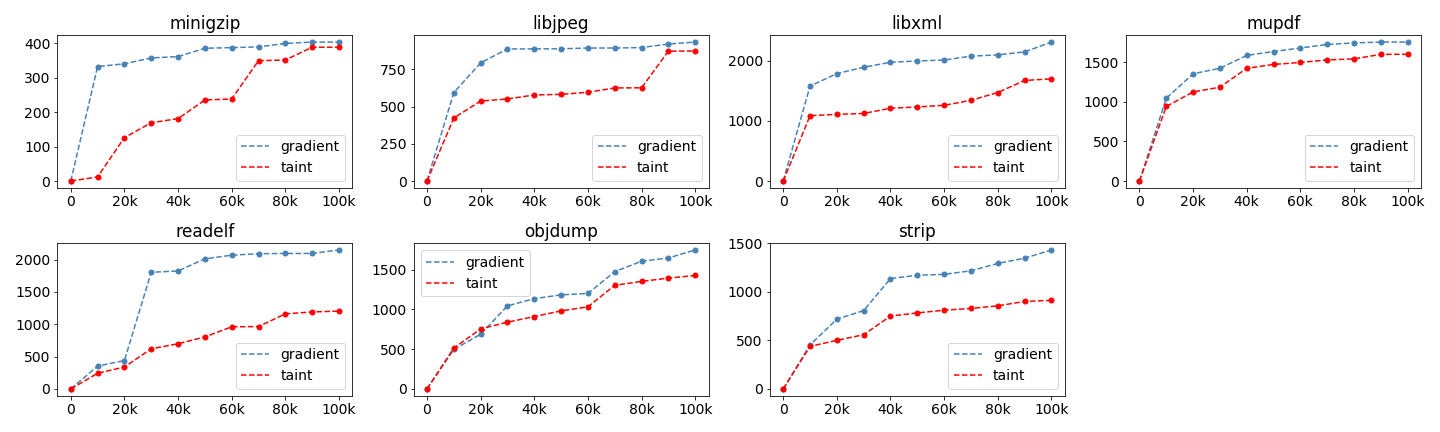
\includegraphics[width=\linewidth]{figs/fuzz_comp_plot}
  \vspace{-10pt}
   \caption{ \label{fig:fuzz_comp}Comparison of guided fuzzer coverage achieved by gradient and taint analysis over 1 million mutations from a single seed.}
  \vspace{-10pt}
\end{figure*}


\begin{table*}[t]
\centering
  \begin{tabular}{l r rr rr} 
 \toprule
    & & \multicolumn{2}{c}{Taint Guided} & \multicolumn{2}{c}{Gradient Guided} \\ 
    \cmidrule(r){3-4} \cmidrule(r){5-6}
    Test Program & Original Edges  & Final Edges & \# Executions &  Final Edges & \# Executions\\ 
 \midrule
   minigzip (zlib-1.2.11)  &      &  &  &  &   \\ 
   mutool (mupdf-1.14.0)   & 2114     & 3509 & 3667  & 3551 & 3667  \\
   xmllint (libxml2-2.9.7) & 3573      &   4085   & 2400   &   4288   &  2400      \\
   djpeg (libjpeg-9c)      & 1259     & 2067     &   285420    & 2160 & 285420 \\  
   readelf (binutils-2.30) & 1379      & 1609  & 2994 & 1795  & 2994  \\  
   objdump (binutils-2.30) & 2804     & 3167 &3352  & 3426 & 3352  \\  
   strip   (binutils-2.30) & 2603     & 3191 & 3155 & 3624 & 3155  \\  
 \bottomrule
 \end{tabular}
  \caption{\label{tab:fuzzer_comp}Summary of guided fuzzing coverage comparison results for Taint and Gradient Analysis. \gabe{Temporarily keeping this for reference but will replace with figure \ref{fig:fuzz_comp}}}
\end{table*}

\subsection{Bug Finding}

In addition to performing comparative evaluations of gradient with taint tracking, we also evaluate its utility as a tool for finding bugs in real world programs. We test gradient analysis in three applications: detecting attacks at runtime, guiding discovery of new vulnerabilities, and discovering information leaks.


\subsubsection{CVE-detection}

We first evaluate gradient analysis as tool for detecting attacks at runtime, which is the application dynamic taint analysis was originally designed for. To detect the attacks, we instrument the programs so that the gradients of parameters of instructions involved in the attack are recorded. As shown in table ~\ref{tab:cve_detection}, we test X known attacks against all 7 programs and demonstrate gradient analysis can detect all X attacks. This result shows that gradient can perform that same task as dynamic taint analysis as a baseline. \gabe{If we can generate an input that triggers a detectable error by gradient but makes dfsan run out of labels we can also talk about that. }

\begin{table}
\begin{tabular}{l l l}
\toprule
CVE ID & Vulnerability & Program \\
\midrule
CVE-2018-10372 & heap overflow & readelf  \\
CVE-2018-6759 & null pointer dereference & nm  \\
CVE-2018-19932 & integer overflow & strip  \\
\bottomrule
\end{tabular}
\caption{\abhi{TODO}}
  \label{tab:cve_detection}
\end{table}


\subsubsection{Bug Discovery}

After evaluating gradient analysis as a tool for detecting known attacks, we next evaluate the utility of gradient analysis in discovering new bugs in programs. To do so we add additional instrumentation to record gradients for instruction and function arguments that can potentially trigger program errors, such as memory allocations, copy instructions, indexing operations, and shift operators. We then execute the programs on a corpus of files generated by running AFL on each program for 24 hours, as well as a selection of files generated from other programs to further extend coverage. For each file, if any input bytes have a nonzero derivative with an instrumented function, we generate new inputs using the function gradient as a guide. For most functions we generate inputs setting the bytes with a gradient to either 0 or 255, although for instructions can potentially trigger a division by 0 we also search all possible values for each byte.

Table ~\ref{tab:bug_summary} summarizes our results. Overall we find X bugs across all 7 programs, including buffer overflows, memory allocations, integer overflows, and division by 0. \gabe{Discuss these results more when we a better bug count.}

\begin{table}
\centering
 \begin{tabular}{ll l l} 
 \toprule
  Library & Test Program & Arithmetic & Memory \\ 
 \midrule
 zlib-1.2.11    & \verb|minigzip -d| &     &  \\ 
 mupdf-1.14.0   & \verb|mutool show| &     &  \\  
 libxml2-2.9.7  & \verb|xmllint| &     &  \\
 libjpeg-9c     & \verb|djpeg| & 3    &  \\
 %harfbuzz-1.7.6 & \verb|minigzip -d| &  9,853   & TTL \\
                & \verb|readelf -a| &     &3  \\  
  binutils-2.30 & \verb|objdump -xD| & & 1 \\  
                & \verb|strip | &     & 6 \\  
 \bottomrule
 \end{tabular}
  \caption{Summary of bug types found by Gradient Analysis for parser programs.}
  \label{tab:bug_summary}
\end{table}



\subsubsection{Information Leak Discovery}

Finally, we evaluate gradient analysis as tool for discovering information leaks in programs. Side channel attacks that take advantage of information leaks in systems are a common method for bypassing traditional security measures. To evaluate gradient analyis as a method for assessing vulnerability to these types attacks, we... \gabe{I'm not quite sure yet, this will probably involve looking at gradients to branches or memory allocations from specific fields in the input.}

Table \ref{tab:information_leaks} summaries our results. We find X information leaks in total across Y programs, and use gradient analysis to identify how the leaks occur in the programs. 


\begin{table}
\begin{tabular}{l l l}
\toprule
Program & Leaked Data & Leak Vector \\
\midrule
mutool & content header type & runtime \\
minigzip & compression type & runtime \\
objdump & note header size & memory usage \\
\bottomrule
\end{tabular}
  \caption{\label{tab:information_leaks} Examples of information leaks identified with gradient analysis. \gabe{This is just a filler table.}}
\end{table}


%-------------------------------------------------------------------------------
\section{Related Work}
%-------------------------------------------------------------------------------

\noindent \textbf{Information Flow Analysis} start with information flow, problem that has been studied since 70s (find first paper)

\noindent \textbf{Dynamic Taint Tracking}Introduced in 2004 by Dawn Song to automatically detect buffer overflow attacks and generate attack signatures. Mark inputs and track whether they effect jump pointers, function pointers, etc (Mention why is it better than stack canaries and other static defenses). Problem is initial frameworks didn't handle conditional branching and limited inputs that were marked and sinks, thus overtainting wasn't a problem but missed potential attacks. More recent taint frameworks 2008-2012 (cite minimu, libdft, dytan, sword dft, more?) 

- address iodine

- address taintinduce

\noindent \textbf{Guided Fuzzing} While some fuzzers have used dataflow directly (buzzfuzz, vuzzer), others use methods that are related to gradient. address neuzz, uses neural netowrk to estimate gradients, address angora, uses sampling and coordinate descent. obviously we are different from both, explain how...







%-------------------------------------------------------------------------------
\section{Conclusion}
%-------------------------------------------------------------------------------

In this paper we introduce Proximal Gradient Analysis, a new form of dynamic dataflow analysis that uses proximal methods to approximate gradients over nondifferentiable operations in programs. Gradient analysis is more precise than current dataflow methods and provides more information about program behavior. We provide an implementation of gradient analysis based on the LLVM framework, and demonstrate our implementation performs better than the LLVM implementation of dynamic taint tracking in predicting dataflows and guiding a fuzzer, while adding lower average overhead. Finally, we show gradient analysis is an effective tool for bug finding, detecting X different CVEs, Y bugs, and Z information leaks in 7 real world programs.




\bibliographystyle{plain}
\bibliography{main}

%%%%%%%%%%%%%%%%%%%%%%%%%%%%%%%%%%%%%%%%%%%%%%%%%%%%%%%%%%%%%%%%%%%%%%%%%%%%%%%%
\end{document}
%%%%%%%%%%%%%%%%%%%%%%%%%%%%%%%%%%%%%%%%%%%%%%%%%%%%%%%%%%%%%%%%%%%%%%%%%%%%%%%%

%%  LocalWords:  endnotes includegraphics fread ptr nobj noindent
%%  LocalWords:  pdflatex acks


